\usetikzlibrary{angles,quotes,decorations.pathreplacing}
% 1991_shanghai_q27_fig1: first draft (frozen)
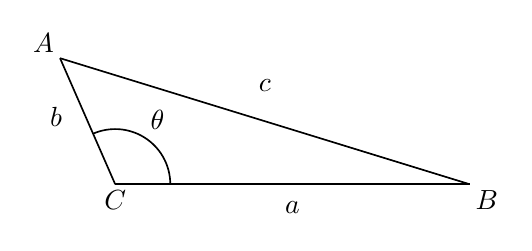
\begin{tikzpicture}[x=1cm,y=1cm,font=\normalsize,
 geometry edge/.style={solid,line width=.6pt},
 geometry mark/.style={solid,line width=.6pt},
 geometry label/.style={font=\normalsize,inner sep=2pt}]
\coordinate (A) at (0.8,1.6);
\coordinate (C) at (1.5,0);
\coordinate (B) at (6,0);
\draw[geometry edge] (A)--(B);
\draw[geometry edge] (B)--(C);
\draw[geometry edge] (C)--(A);
\pic[draw,geometry mark,"$\theta$",angle eccentricity=1.4,angle radius=7mm] {angle=B--C--A};
\node[font=\normalsize] at (3.75,-.3) {$a$};
\node[font=\normalsize] at (0.75,0.85) {$b$};
\node[font=\normalsize] at (3.4,1.25) {$c$};
\node[geometry label,above left] at (A) {$A$};
\node[geometry label,below] at (C) {$C$};
\node[geometry label,below right] at (B) {$B$};
\end{tikzpicture}
